\chapter{関連研究}
\label{chap:webapi}

本章ではユーザーの仮想現実や明晰夢における認識度や要求について事前調査、睡眠に関する調査、睡眠中に見たい夢の分析を行った。そしてDreamDateの開発に反映した点について述べる。

\section{仮想現実システムに関するアンケート調査}
人がどのような仮想現実を望んでいるかを調査するため、理系の学生7人、文系の学生7人、サラリーマン10人、主婦3人を含めた20〜60歳の男女27人にオンラインアンケートをした。これらのインタビュー結果を経て一般的なユーザのニーズを把握し、DreamDateの有効性やDreamDateが解決すべき問題について明らかにする。

%\subsection{仮想現実を体験するために一般的な人々が支払う金額}
%各所公式ウェブサイトを掲載し、機能性やデザインの詳細を説明した上で、仮想現実を見る手段として次の選択肢から購入しようと思う商品を選んでもらった。

%\begin{itemize}
%\item OCULOUS Rift:85278円
%\item ハコスコ:1500円
%\item iWink:36478円
%\item タカラトミー夢見工房:15984円
%\item DreamDate :無料
%\end{itemize}

%すると図\ref{userNeedCost}のように、一般ユーザーの中には仮想現実を体験するためにOCULOUS Riftなどの高額なデバイスを購入しようとする人は少ないということが分かった。1500円ハコスコだと少し数が増えるが、これらのデータから無料で簡単に手に入れることができるツールを多くの人が必要としていることが示唆された。

%\begin{figure}[htbp]
%\begin{center}
%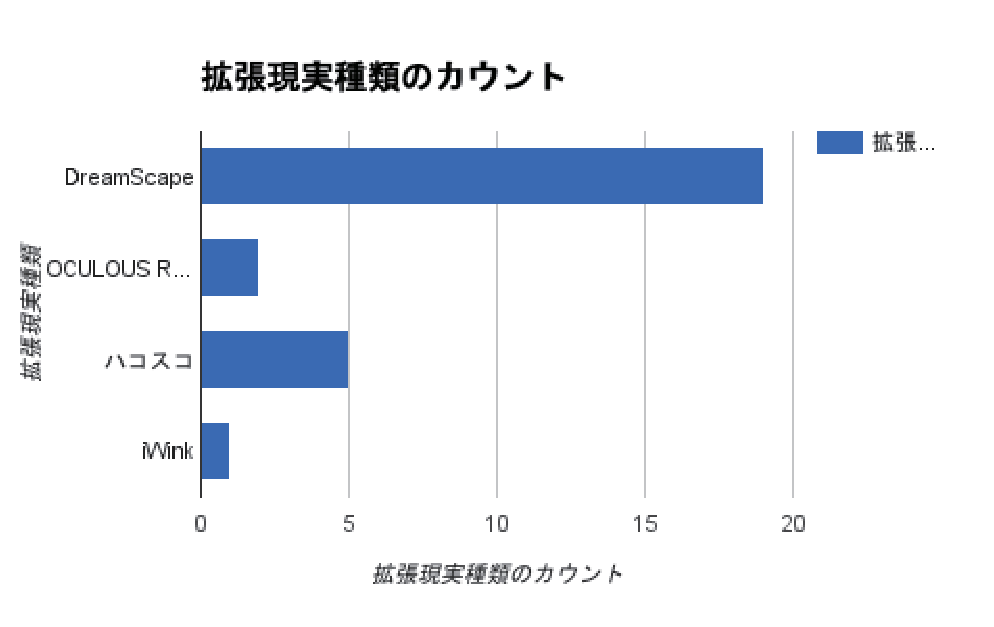
\includegraphics[width=15cm]{eps/VRselection.eps}
%\caption{仮想現実を体験するために一般的ユーザーが選ぶデバイス}
% \label{userNeedCost}
%\end{center}
%\end{figure}

\subsection{仮想現実を体験したいタイミング }
仮想現実を体験したいタイミングとして、睡眠中と起きている時間帯でどちらが好ましいかについて調査を行った。すると睡眠中と答えたのは52\%、起床中と答えたのは48\%。このように結果にはあまり差がなかった。睡眠中を選択した人は理由として「睡眠時間の有効活用のため」と答えた。比べて起きている時と選択した人は「起きたら忘れてしまうかもしれないから、意識のある時に体験したい」と答えた。よってDreamDateの開発において、睡眠中の体験がユーザーにどのような印象を与えるかを研究することは意義があると考えられる。

\section{夢と睡眠}
睡眠中に扱うアプリケーションの開発にあたって、睡眠自体を理解することは不可欠である。事前調査によって明らかになった睡眠段階や夢についてここで記す。

\subsection{夢と記憶}
夢は空間、時間軸と、登場人物が非現実的な場合など不合理で異様な内容のことが多いが、大抵の場合人は、現実だと錯覚し夢を見ていることに気がつかない。それは論理的思考力を担う前頭前皮質の機能が低下しているためだ\cite{cortex}。起床後も夢での感情が現実で起きたかのように勘違いしてしまうほどリアルな体験をする人も多い。起床後すぐに夢日記をとれば、本当の思い出のように夢の記憶が残る場合もある。
 心理学者であるSigmund Freudは1905年に無意識の欲求や感情、抑圧された子供の頃の記憶、生理的欲求などが夢に大きな影響を与えていると述べた\cite{freud}。一方で2006年にJie Zhangは夢は短期的な記憶を長期的な記憶に変換するためのプロセスであると述べている。この図\ref{brainZhang}は睡眠中の脳の働きを表す\cite{Zhang}。脳の容量には限度があるため、睡眠中に過去の記憶の中で関連性の強い記憶を繋げたり、重複している内容や必要のない記憶を消しているのだ\cite{Zhang}。睡眠時間が減ると暗記能力が減るのもこれにより説明できる。\\
 幼児の平均睡眠時間は16時間でそのう内の50\%をREM睡眠が占める。一方成人の平均睡眠時間は7時間でREM睡眠も短いため、夢をあまり見なくなる。年齢が若いほどREM睡眠の周期が長いのは、経験すること全てが新しいため多くのことを記憶しなければならないことと、脳の空き容量が多いためと説明されている。

\begin{figure}[htbp]
\begin{center}
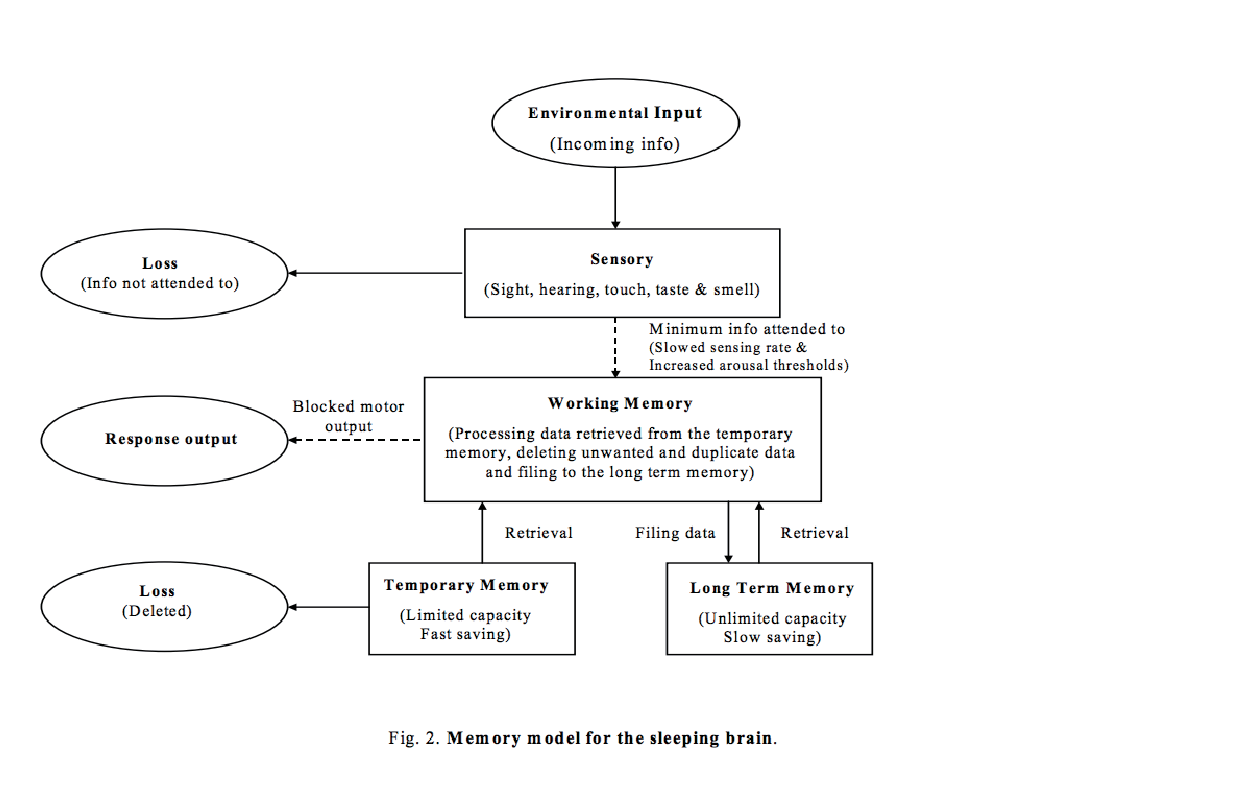
\includegraphics[width=15cm]{eps/sleepBrainModel.eps}
\caption{nonREM睡眠とREM睡眠}
\label{brainZhang}
\end{center}
\end{figure}

\subsection{睡眠と睡眠段階(睡眠の深さのレベル)}
 睡眠は身体を休めるためにある。そして人生の1/3を占める活動である。そして睡眠中人は2つの睡眠段階、レム睡眠とノンレム睡眠を90分間隔で行き来している\cite{Dement}。筑波大学と理化学研究所の研究によるとREM睡眠中は記憶形成や脳機能回復の作用がある脳波(デルタ波)が多く見られるというのが通説である\cite{tsukuba}。そしてレム睡眠中は心拍数や眼球の運動が活発化する。レム睡眠の最中に起きたときは夢も比較的覚えているという研究もされている\cite{remNonRem}。一方ノンレム睡眠中は脳も身体も休んでいる。\\
 図\ref{SleepHypnogram}は平均的な睡眠のサイクルを示したものである\cite{hypnogram}。睡眠に突入して初めてのレム睡眠は10〜12分でもっとも短い。2度目のレム睡眠は15〜20分。最後の夢は15分であるが、通常はアラームなどによって不意に中断されることが多い。平均的に一晩で5〜7回夢をみる。一般的な人生で人は6年間夢を見る。DreamDateはこの6年間をより充実感のある体験にするために貢献できるアプリケーションになる可能性があるのだ。

\begin{figure}[htbp]
\begin{center}
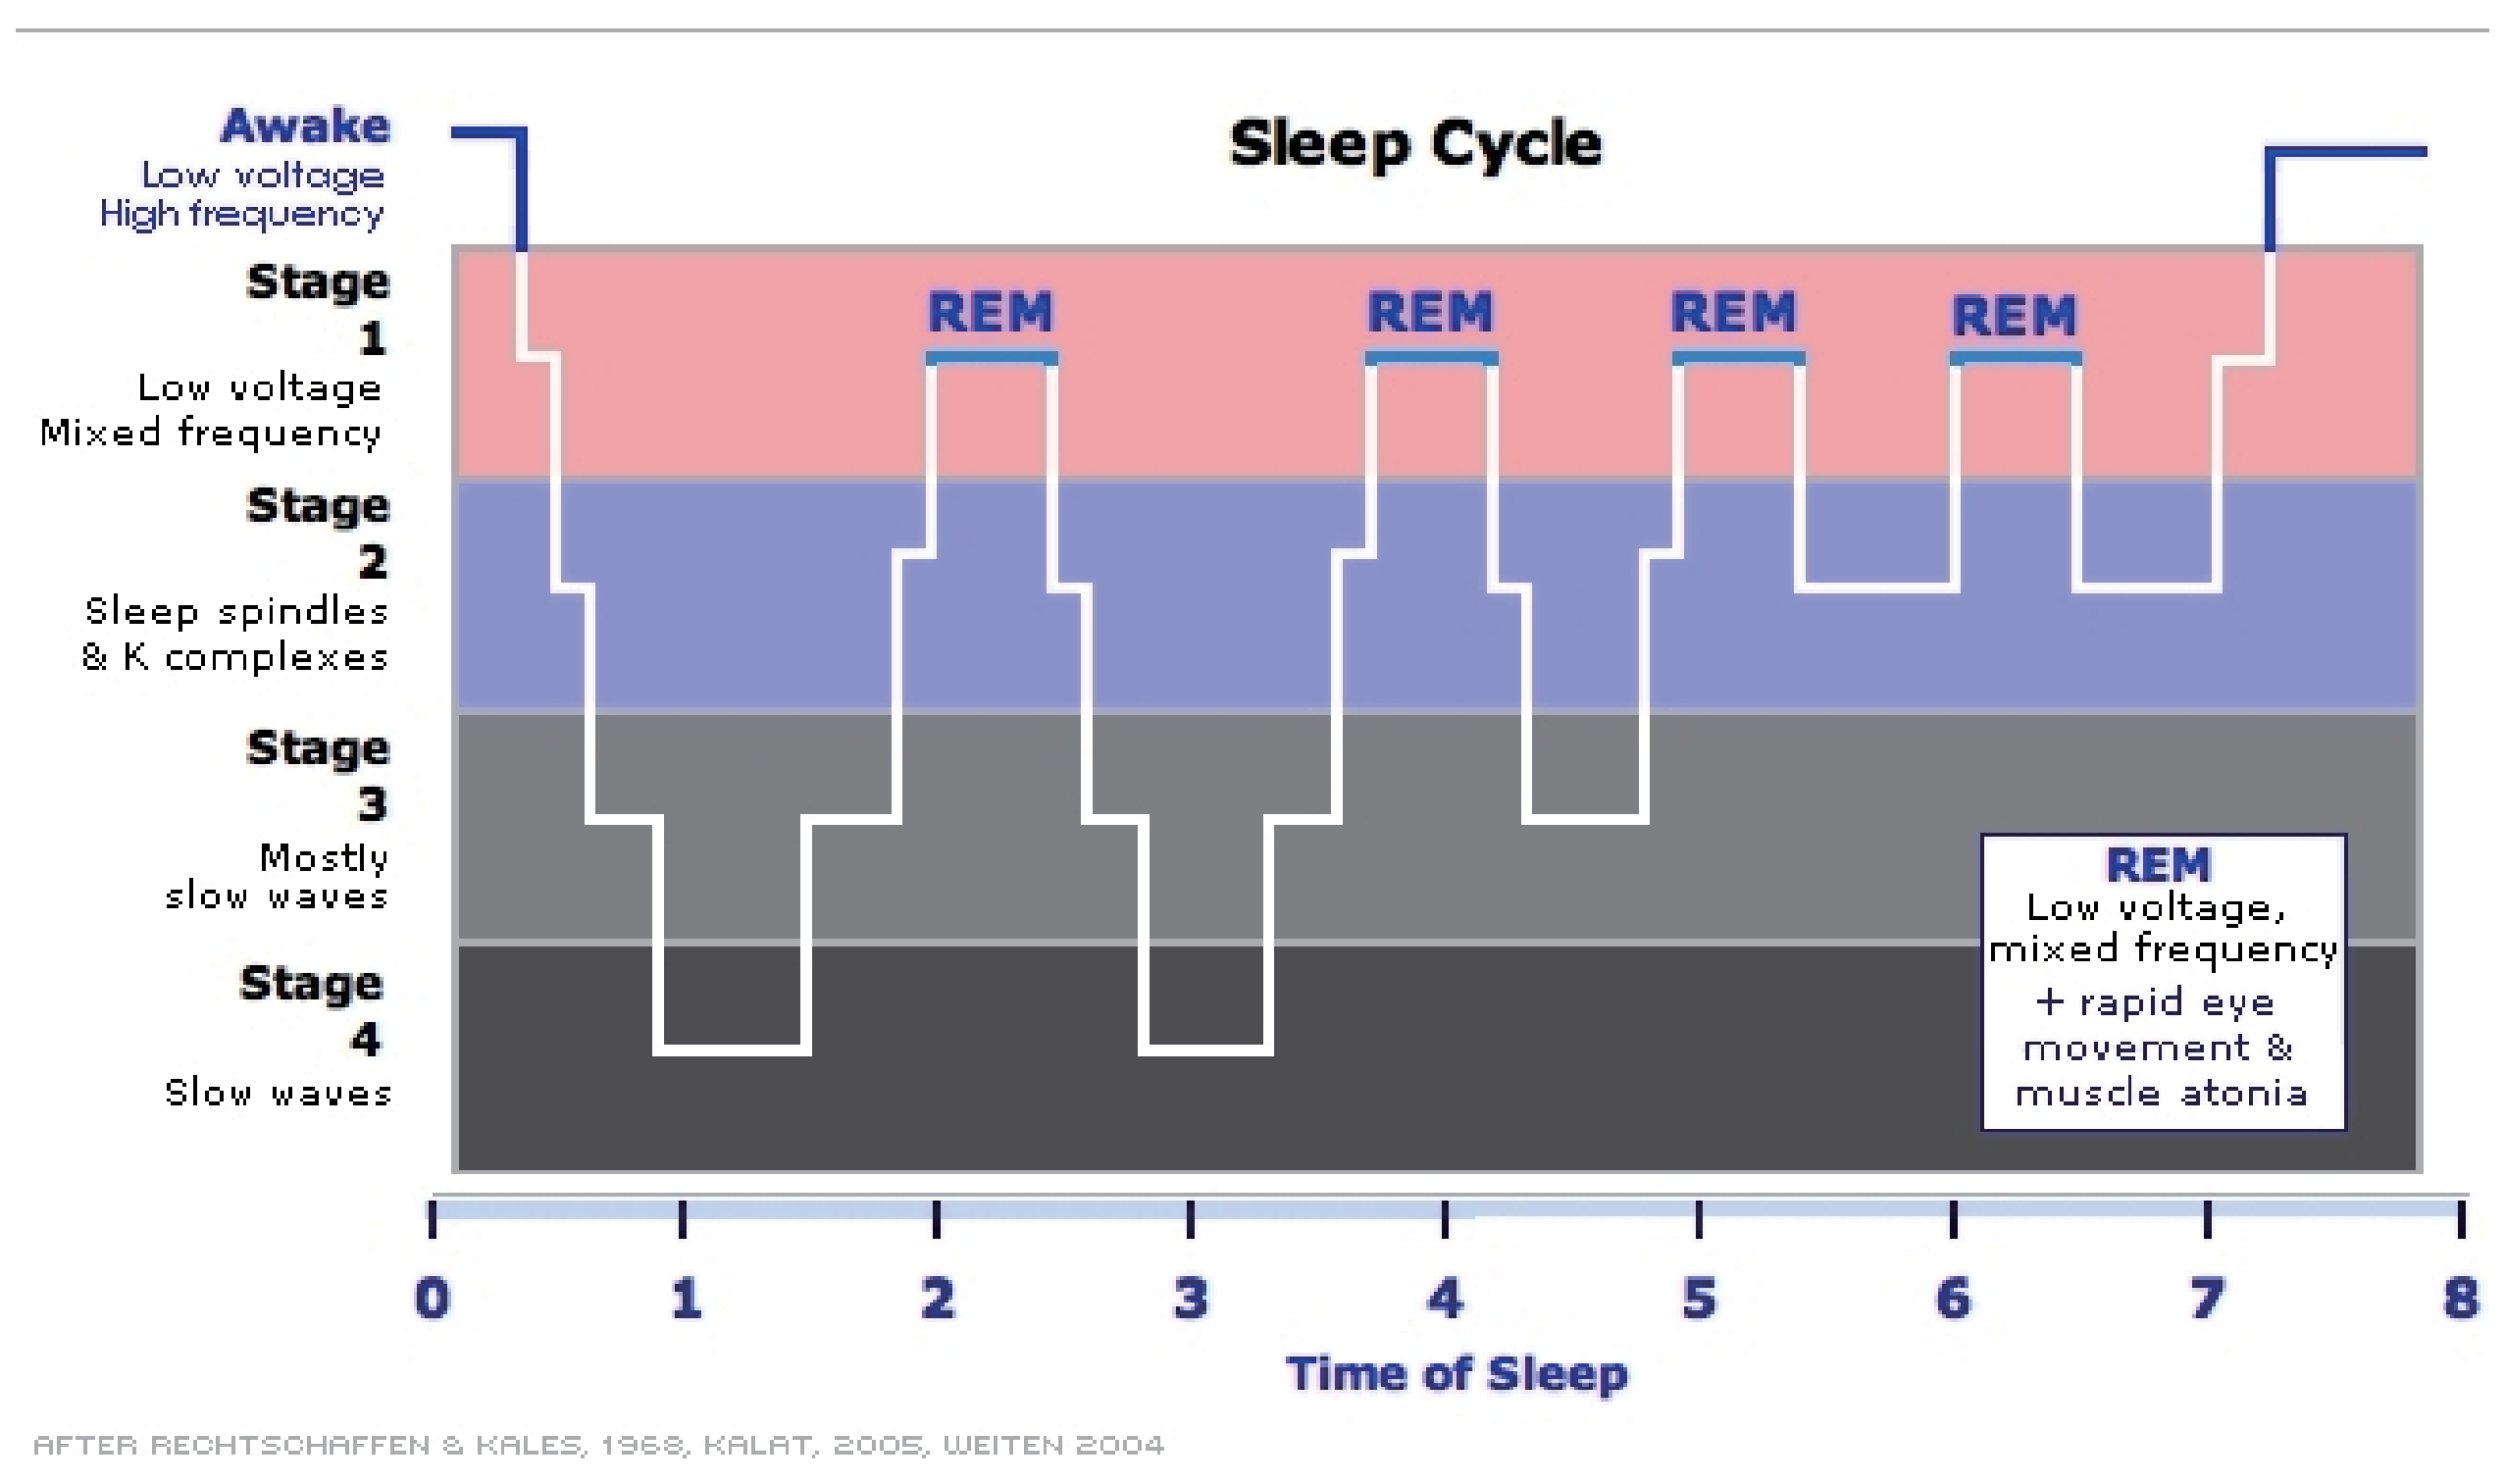
\includegraphics[width=15cm]{eps/SleepHypnogram.eps}
\caption{REM睡眠中の脳の働きのモデル}
\label{SleepHypnogram}
\end{center}
\end{figure}

\subsection{睡眠段階のセンシング方法}
睡眠段階のセンシング方法として正確性が高いのは脳波センサーである。しかしそれ以外のセンシング方法もある。人はREM睡眠中に眼球が活発化し心拍数が多少上がるので、眼球の運動と心拍によりセンシングが可能である。人は睡眠段階を移行させるために寝返りを行う習性があるとされている。要するに睡眠サイクルのスイッチのような働きをするのだ。\cite{negaeri}よって寝返りをモニタリングすれば睡眠段階をある程度センシングすることが可能であるということが通説である。

\section{明晰夢に関するアンケート調査}
夢の操作に成功したとしてもその夢を覚えていなければ意味がない。そこで実験を始める前に一般的に人は夢の内容を起床後どのくらい覚えているのかをアンケート調査した。夢をよく覚えていると答えた人は内容によっては覚えていると答えたのは10人、覚えていないとこ答えたのは13人、よく覚えているのと答えたのは4人であった。
%\begin{figure}[htbp]
%\begin{center}
%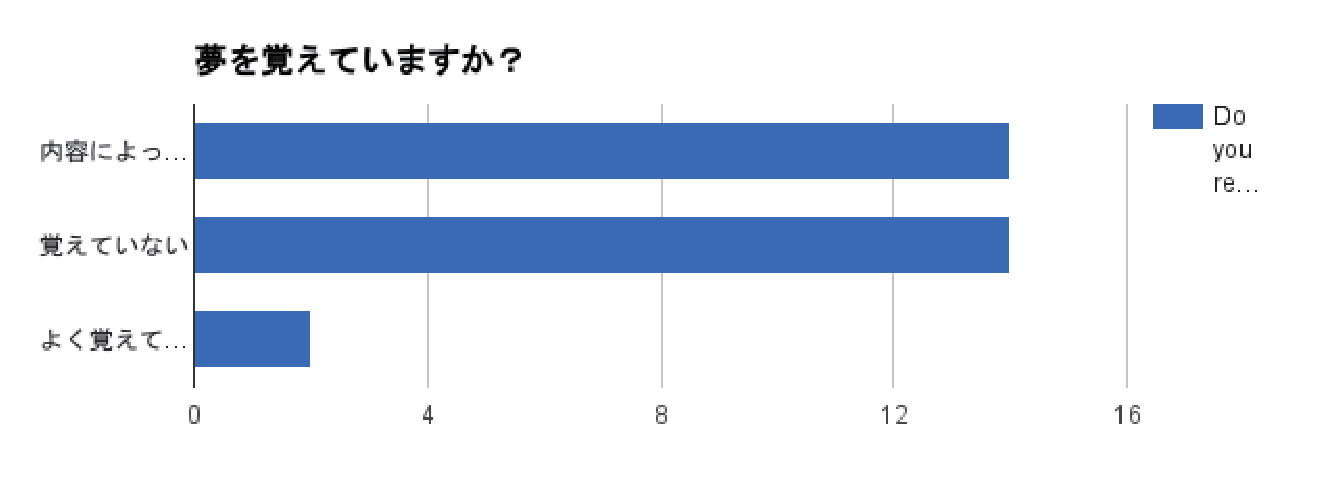
\includegraphics[width=15cm]{eps/remember.eps}
%\caption{夢を覚えている比率}
%\label{rememberDream}
%\end{center}
%\end{figure}

覚えている夢は刺激的、怖い夢、繰り返し見た夢というのが多く、日常的な夢は忘れがちであるということが分かった。人は睡眠中の夢の90\%を起床後5分間で忘れるという。Jie ZhangによるとREM睡眠中は短期的な記憶を担っている脳は長期的な記憶への移行に注力していて、インプットの部分があまり機能していないためであると説明する\cite{Zhang}。ただ起きてすぐに夢日記で夢を記憶すれば覚えていられることが可能なのだ\cite{forgetDreams}。\\

Sigmund Freudは「夢判断」の中で人は睡眠中の姿勢、環境、身体的刺激によって夢の内容が変化すると述べた\cite{freud}。睡眠中の人間の鼻先を羽毛でくすぐったときに、夢の内容に変化があったことを確認する実験を紹介している。そこで音、体制、匂い、振動、光、などの刺激の中で何が夢に一番影響を与えやすいのかを男女27人にオンラインアンケートをとった。以下の図\ref{externalShigeki}がその結果を示す。音が他の刺激よりも影響を与えやすいということが分かった。また学術的にも聴覚と嗅覚は人間の生命維持を高めるために感度は低いが睡眠中も機能しているということが証明されている\cite{Zhang}。\\

\begin{figure}[htbp]
\begin{center}
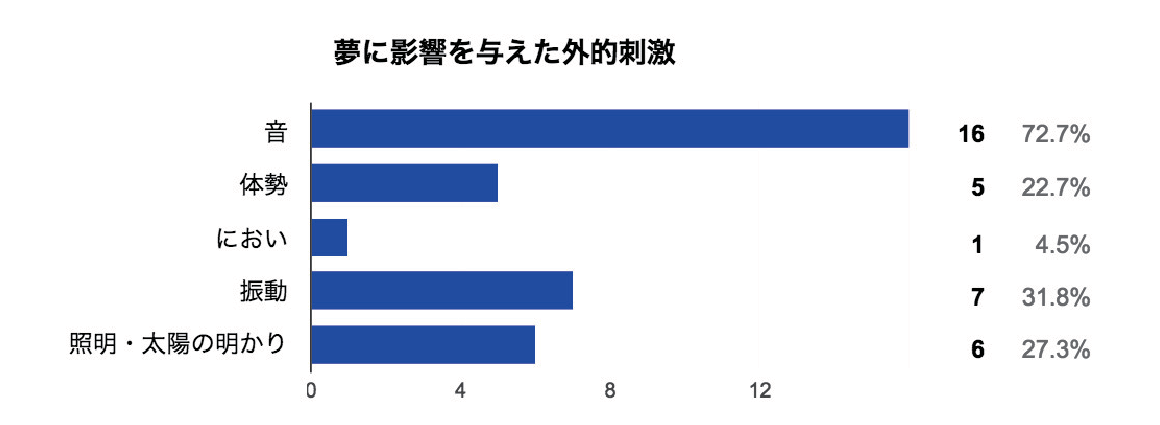
\includegraphics[width=15cm]{eps/input.eps}
\caption{夢に影響を与えた外的刺激}
\label{externalShigeki}
\end{center}
\end{figure}

明晰夢を体験したいか否かで質問をしたところ77\%の人が体験したいと答えた。仮想現実で体験したい内容を調査結果から似ているものをカテゴリー別に分けて、図\ref{desiredDreamTpye}で示した。LOVEタイプ、癒しタイプ、元気欲しいタイプ、アドベンチャータイプ、ストーリータイプ、ビジネスタイプとあるがそれぞれの定義を述べる。LOVEタイプとは恋愛や性的行為などが含まれる内容。アドベンチャータイプは冒険など非日常の体験を求める内容。ストリータイプはドラマのように連続性のある夢を求める内容。癒しタイプ・元気欲しいタイプは娯楽を求める内容。原強化タイプは睡眠中になんらかの学習を求める内容だ。LOVEタイプと癒し・元気が欲しいタイプが最も多く、少数派としてビジネスタイプがあった。\\

\begin{figure}[htbp]
\begin{center}
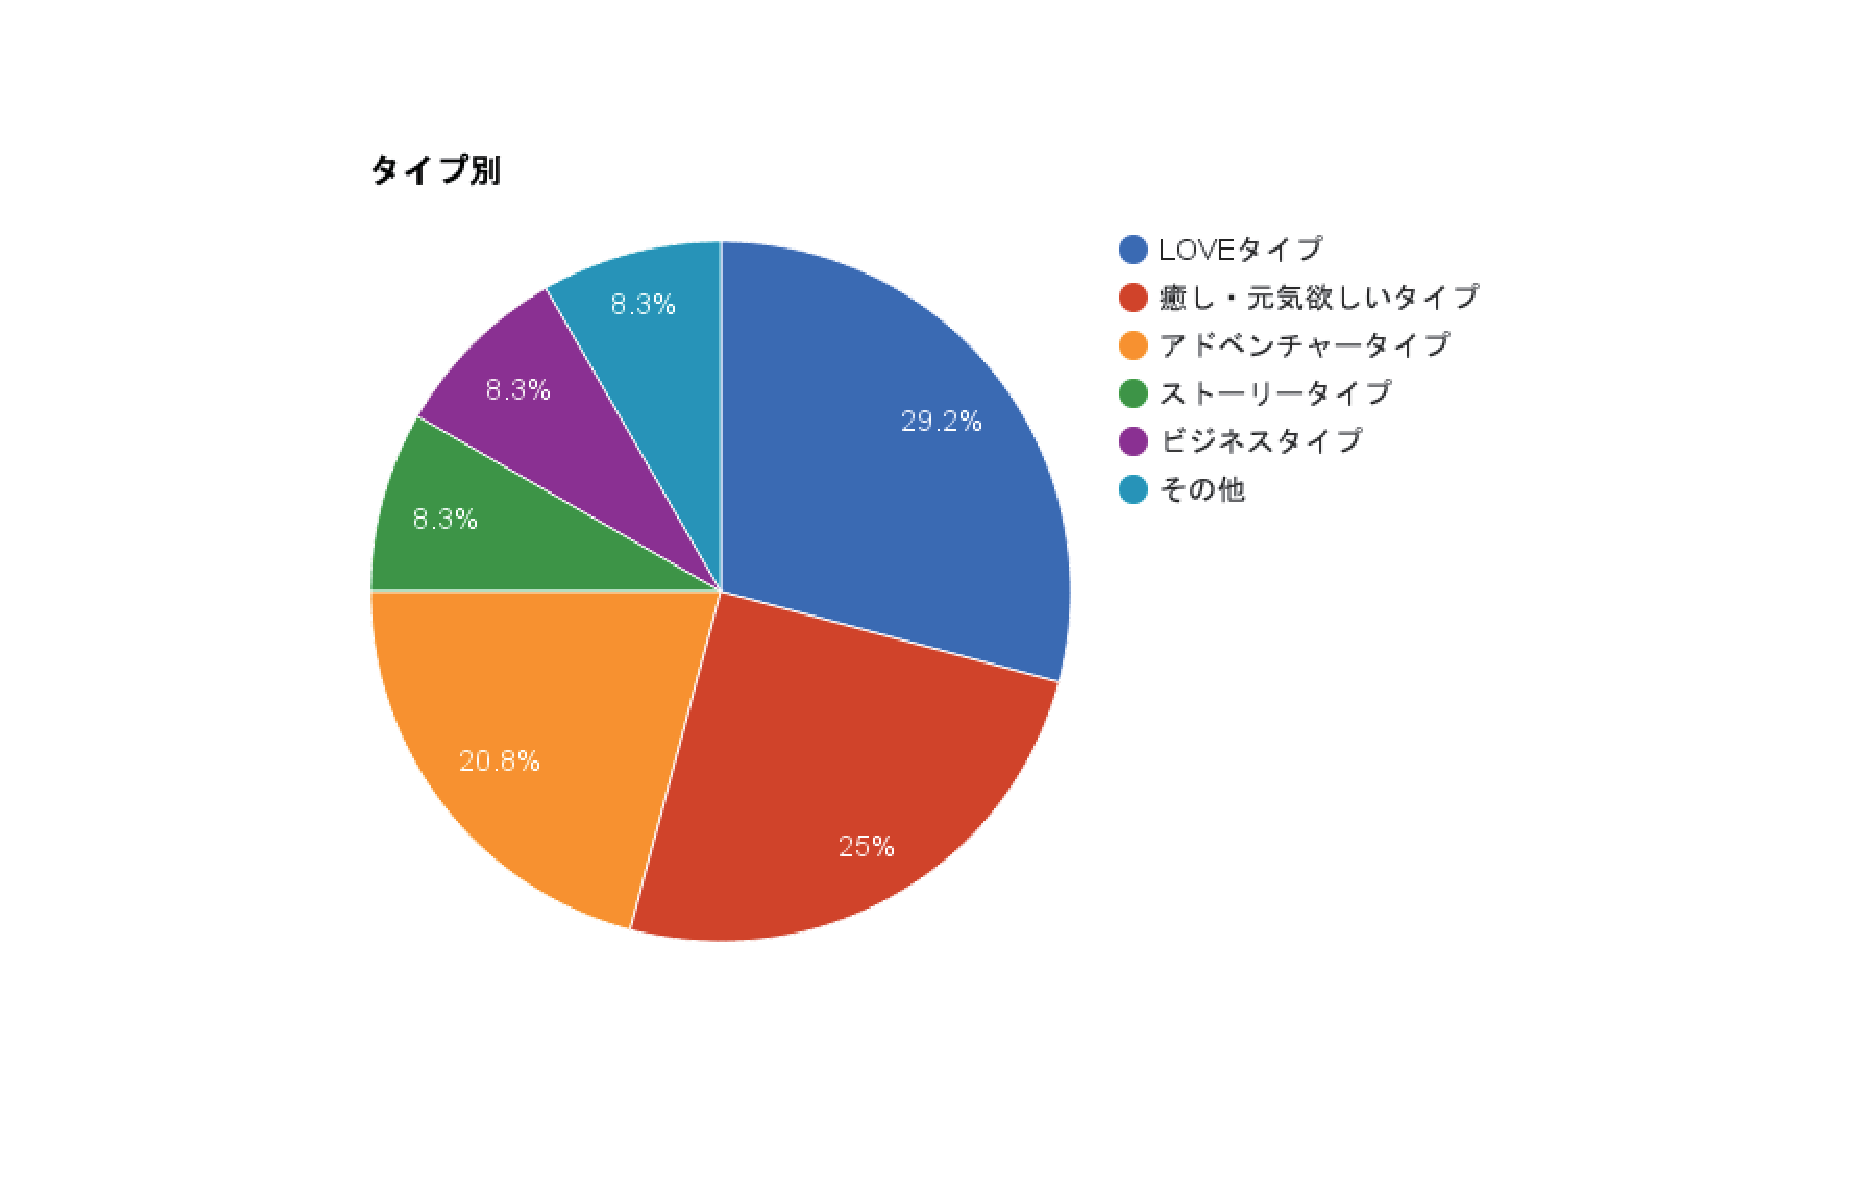
\includegraphics[width=15cm]{eps/dreamType.eps}
\caption{明晰夢で体験したい内容のカテゴリ:分析1}
\label{desiredDreamTpye}
\end{center}
\end{figure}

回答をさらに違った方法で分析した結果が\ref{desiredDreamTpye2}である。これらの結果からユーザーによって理想の夢は日常や非日常、具体性や抽象性に隔たりがあり、一貫性が見られないことがわかった。
\begin{figure}[htbp]
\begin{center}
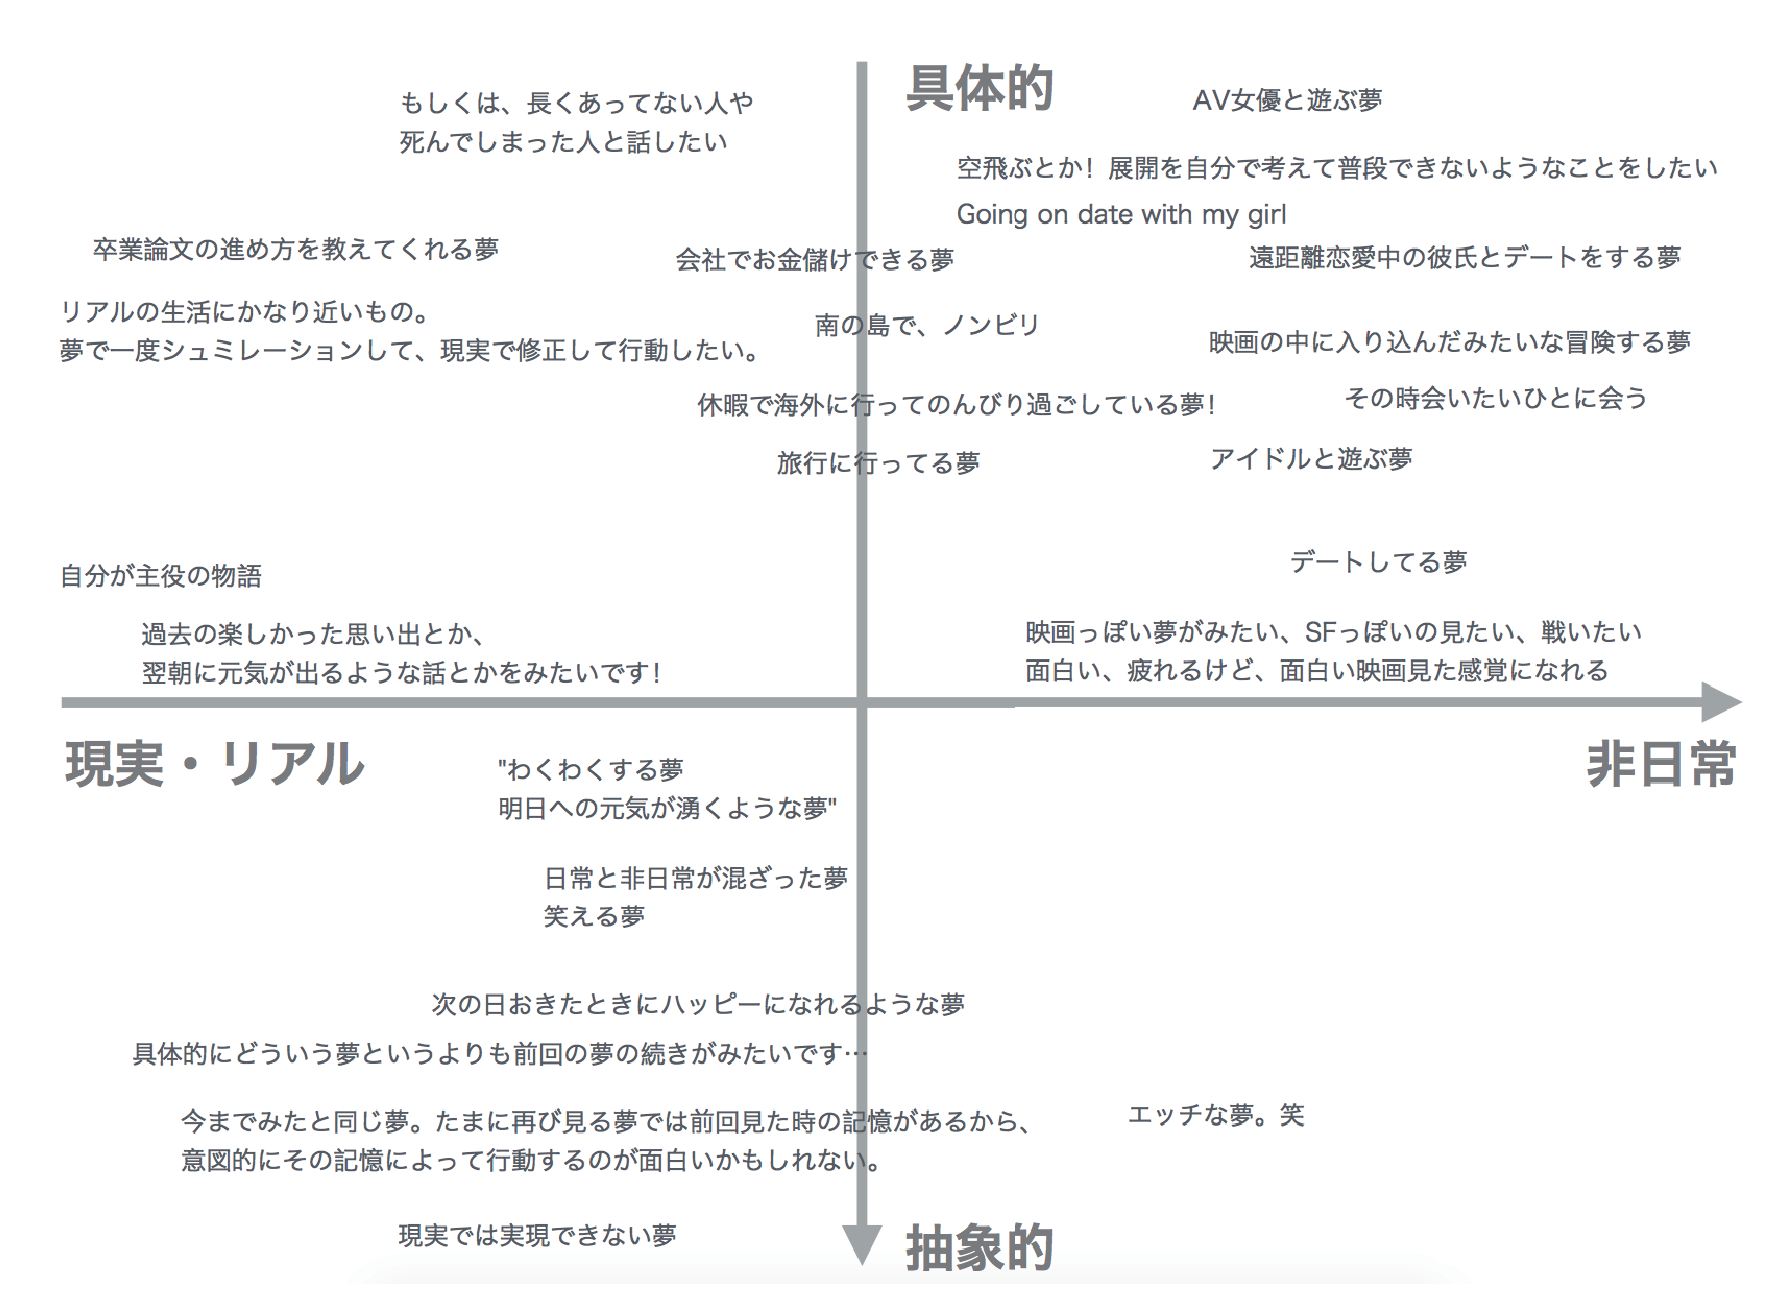
\includegraphics[width=13cm]{eps/whatYouWantToDream.eps}
\caption{明晰夢で体験したい内容の詳細:分析2}
\label{desiredDreamTpye2}
\end{center}
\end{figure}

\section{睡眠の観測と夢の制御}
\subsection{睡眠の観測}
DreamDateは睡眠中に仮想現実を体験するための手段として考えられた研究である。よって正確に睡眠をモニタリングする方法を探究するというのはこの論文の主旨ではない。しかし明晰夢に影響を与えるのに夢をみる時間帯であるREM睡眠を観測することは重要な鍵となる。以下にモニタリングに注目した先行研究を紹介する。

Bedditは睡眠の質を向上させるためにセンサーで情報を蓄積してアプリでユーザーに情報を共有するために作られたデバイスである。マットの上にセンサーを配置、鼓動によって起きる血流の変化と呼吸に伴う肺の動きをセンサーで観測をしている。ウェラブルデバイズではないためユーザーが使用しやすいが、デバイスが18966円と高額である。
%\item 正確性:46人を対象に実験し、心電計と比べた結果bedditの結果が99.94%の相関性があると証明されている
%\item 値段:18966円

株式会社オムロンが開発したねむり時間計は、枕元に置くだけで電波センサーが睡眠時間を測定する。測定結果がスマートフォンに転送されて、アプリで睡眠の質(寝返りの回数など)や時間を一週間単位で分析できる。ユーザーに適した睡眠効率向上のアドバイスする。電波センサーでモニタリングが行われる\cite{omron}。プロダクト自体デザインやアプリのユーザーインタフェースへのこだわりが評価され2012年に『グッドデザイン賞』を受賞している。
%\item 正確性:商業目的の製品のため詳しいデーターは明かされていない
%\item 値段:3630円

\begin{figure}[htbp]
\begin{center}
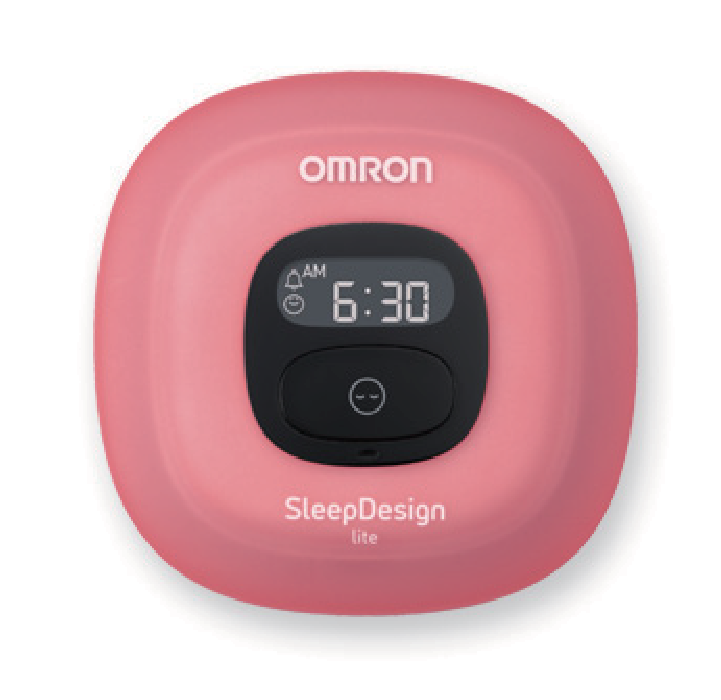
\includegraphics[width=7cm]{eps/omuron.eps}
\caption{オムロン睡眠計の外観}
\label{omuron}
\end{center}
\end{figure}

neuroonは睡眠サイクルの改善、光セラピーのためのウェラブルマスクである。脳波、眼球の動き、心拍数、血液中の酸素量、加速度、体動と体温全てのセンサーが搭載されている\cite{neuroon}。脳波を含んでいるということで正確性が高いのが特徴である。
%\item 正確性:商業目的の製品のため詳しいデーターは明かされていない
%\item 値段:36478円

Zeroは睡眠時無呼吸症候群の解決などを目的としたウェラブルデバイスである \cite{beWellApp}。脳波センサーにより睡眠の各ステージを正確に突き止めることができ、正確性は高い。しかし頭に装着しなければならないデバイスなので汗をかきやすくなり、ユーザーの負担になるので長期的な利用には向いていない。

iSleepは健康向上のために睡眠時間とその質をスマートフォンのアプリである。スマートフォンに備わっている音声録音機能で体動、咳やいびきなどを測定\cite{iSleep}。アプリをダウンロードするだけで簡単に使えるが特徴だ。ローンチ10日間で100人のユーザーから睡眠に関する詳細なデータを集めている。
%\item 値段:361円
%\item 正確性:被験者7人51日間の睡眠で90\%の正確性

BeWellAppもうつ病、心配性、不眠症、高血圧になりにくい生活習慣へ導くために睡眠の長さを測るスマートフォンのアプリである。しかしユーザーによるインプットは一切必要なく、ユーザーの充電、加速度からスマートフォン利用頻度・時間を測定、静けさ、部屋の明るさなどから、睡眠スタイルを検知する仕組みになっている\cite{beWellApp}。アプリという形で多くの人に実験をしてもらえる、ユーザーは普段の生活となんら変わりなく、過ごせるため、負担がかからないのが特徴だ。
%\item 効果:8人の被験者に、Jawbone、Zeoと、BESモデルのアプリを試してもらい、全ての人がユーザー体験を過ごせたと結果がきた。
%\item 正確性:睡眠時間+-42分
%\item 値段:商業用目的ではないため不明

以上の先行研究を踏まえると、睡眠の感知の仕方は様々であるということがわかる。最も正確であるとされているのは眼球の動きをトラッキングする手法と脳波センサーであるが、これでは身につけるタイプのセンサーなのでユーザーの負担になってしまう。またデバイスを購入するためのコストがかかってしまうので、本論文の主旨とずれてしまうことになる。次に体動検知のために使われる電波センサーであるがこれもデバイスの購入を必要とする。そこでもっともユーザーの負担ならずに正確性も証明されているのがiSleepをはじめとするスマートフォンアプリケーションだ。こられの理由からスマートフォンアプリケーションが問題解決の手段としてもっとも適していると判断した。そこでiSleepで紹介されているアルゴリズムを参考にしたプログラムを製作した。

\subsection{睡眠時の刺激提示}
 外的刺激を与えることで睡眠に影響を与えようとした研究や製品開発は前例がある。首都大学の長塚麻美らによる研究では睡眠深度に即した光の刺激を与える抱き枕型のインタフェースを提案している\cite{sleepSheep}。寝付きやすくするために赤に近い黄色の光を点灯させ、波の音を再生するというシステムであるがその実験結果は明らかにされていないためさらなる実験が求められる。\\
 株式会社タカラトミーが開発した夢見工房は音、香り、視覚的情報により夢をより理想的なものに近づけるデバイスである。具体的にはユーザーが寝る前に「恋愛」、「勇気」や、「冒険」からみたい夢のテーマを選び、睡眠時にそれに紐ずいた音楽と香りが発生する。またボイスレコーダー機能もついており、みたい夢を暗示する声が目覚めない程度の小さな音量で自動的にリピート再生させることもできる。 \cite{takaratomi}このように多くの機能が備わっており、気分転換や充実した楽しい時間を作り出すことを目的としているが、正式な効果は発表されていない。また香りや音声の種類に限りがあることや香り製造機の騒音が問題としてあげられている。値段も14,800円と高めである。
\begin{figure}[htbp]
\begin{center}
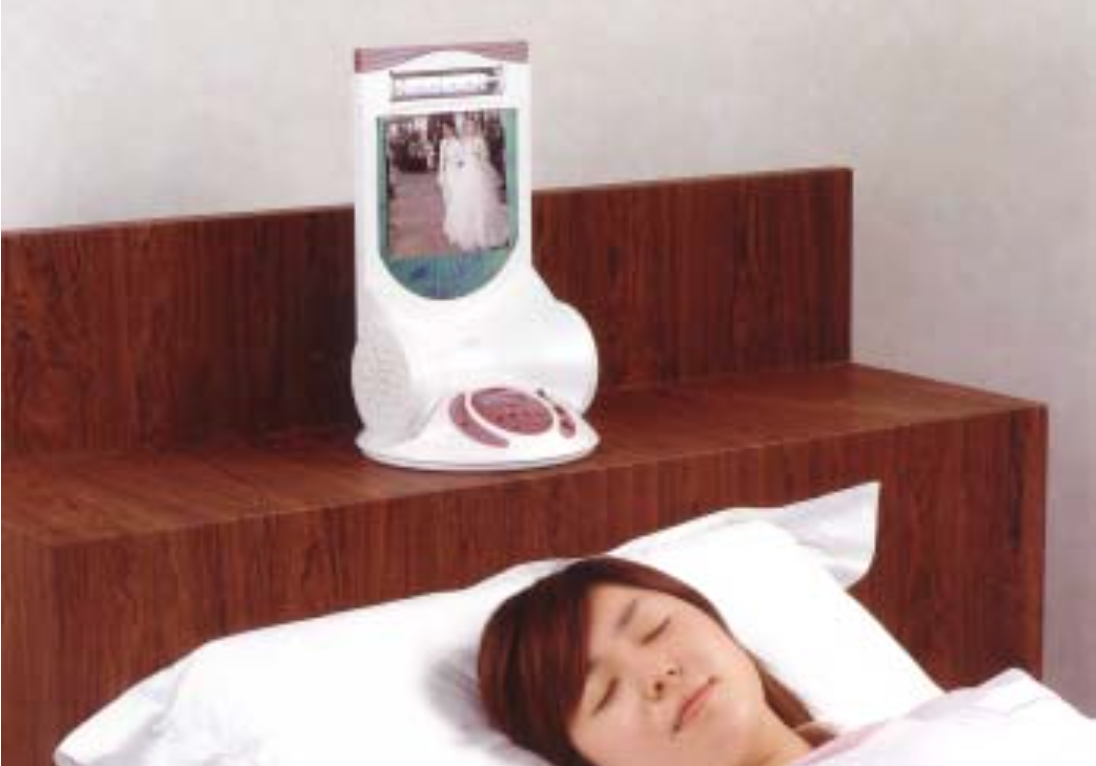
\includegraphics[width=14cm]{eps/takaratomi.eps}
\caption{夢見工房}
\label{takaratomi}
\end{center}
\end{figure}

 他にも明晰夢を促進するとためのツールとしてiWinksにより開発されたAURORAがある。\cite{iWinks}これはレム睡眠時に光による刺激を与えることで、ユーザーに夢を見始るという暗号を送って明晰夢を促すデバイスである。脳波センサー(EEGセンサー)と加速度センサーが組み込まれており、睡眠の質観測においてはクリニックにより検証されたものとウェブページ上には書かれている。しかし明晰夢への効果に関する実験結果が明らかになっていないので、真実であるという確証はない。値段も3,6000円と非常に高額である。\\
 スマートフォンアプリ部門ではDreamOnがある。睡眠中に音楽を流すことで夢に影響を与えるアプリだ。アプリという形で多くの人に夢の研究に参加してもらい音が夢に影響を与えるのか否かについて判明することを目的としている \cite{dreamOn}。ウェブサイトには睡眠は外的刺激に影響を受け、森林の音を流すと夢の中に緑が頻繁に現れて、街中の音を流すと奇抜な夢を見ると書いてある。しかし実験結果についてはかなり疑わしい。App Storeでユーザによる評価は385人によってレーティングが行われており、評価は5点中3である。下記の画像\ref{DreamOnImage}はユーザーのレビューである。悪夢を見たなどの睡眠被害を訴えるレビューが多く見受けられた。DreamOnの他にもユメミール \cite{yumemiru}やDreamDream \cite{DreamDream}など国内のアプリもあるが、どれも信ぴょう性のある実験結果は公開されていない。

\begin{figure}[htbp]
\begin{center}
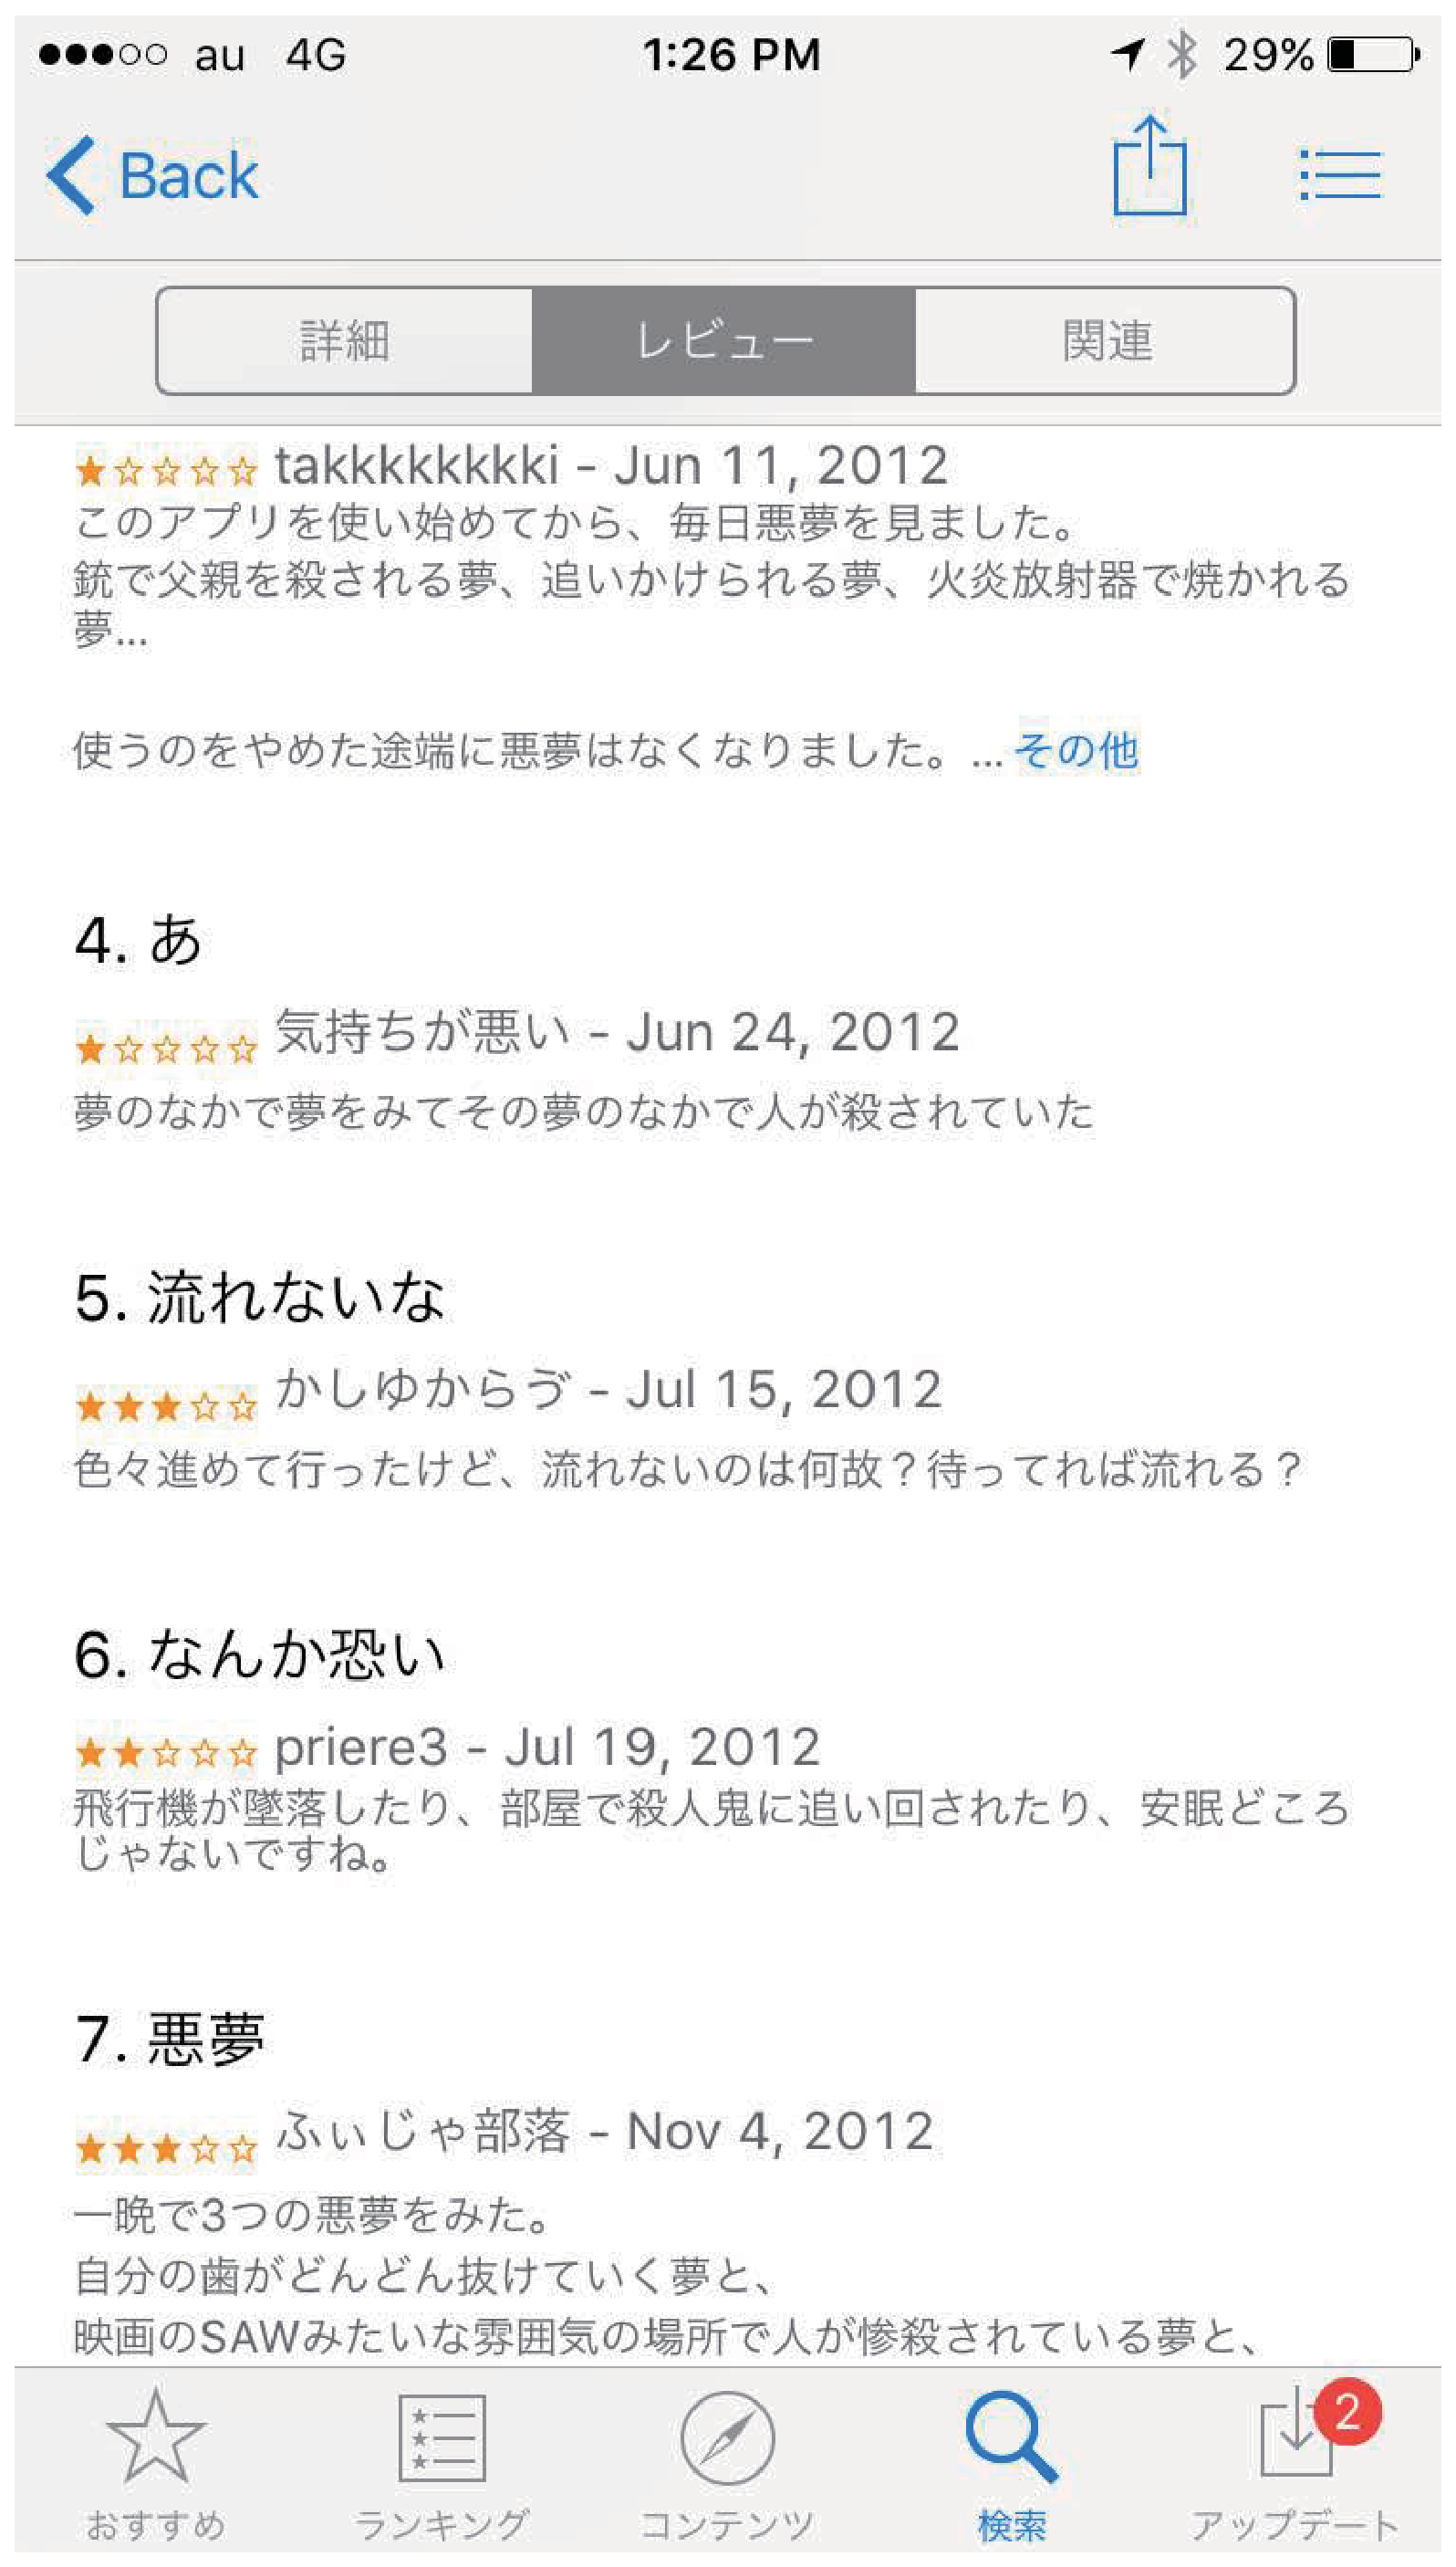
\includegraphics[width=5cm]{eps/dreamOn.eps}
\caption{DreamOnのユーザレビュー}
\label{DreamOnImage}
\end{center}
\end{figure}

\section{本研究の位置付け}
Head Mounted Display(HMD)は仮想現実を体験するためにメジャーな手法として注目を浴び、開発が進んでいる。しかし体験をするためにはOCULUSを始めとした高価なデバイスを購入しなければならない。3 次元のコンテンツを作成するには技術やコストが高くユーザが望むコンテンツを気軽に作れるようにはなっていない。

そこでDreamDateは明晰夢に着目した。明晰夢は睡眠という習慣をより有効に活用し、金銭的コストをかけることなく遂行することができる。1章でも紹介したが明晰夢を体験するためのステップとしてMnemonic Induction of Lucid Dreams (The MILD Technique)がある。しかしThe MILD Technique には労力が必要で誰もが気軽に始められるものとは言い難い。HMDのように金銭的負荷はかからないが快適なユーザー体験ではない。DreamDateはMILDよりにも簡単に使い始められるように、スマートフォンアプリによってユーザーのサポートをする。夢を忘れない体質になるためにThe MILD Techniqueのステップの1つとして紹介されている夢日記をアプリの機能に組み込んだ。

また明晰夢を促進するシステムとして株式会社タラトミーによる夢見工房やDreamONなどのスマートフォンアプリなどが開発されているが、実験結果については明らかになっていないのが現状だ。これらの多くはレム睡眠を検出して音声や香りによる刺激を与えることで夢に影響を与えるシステムだ。DreamDateの開発を通してどのような刺激の与え方最も有効的なのかを調べる。詳細は第3章と第4章で述べる。またDreamDateはbeddit\cite{beddit}、Bed Prssure MatやiSleep\cite{iSleep}などのように睡眠モニタリングデバイスを参考にしてモニタリングシステムの構築をする。

DreamDateシステムに求められる要件:
\begin{itemize}
\item 明晰夢で仮想現実を体験できる
\item ユーザ一人一人の要望に合った音を選ぶシステム
\item HMDのように高価なデバイスを必要としない
\item MILD Techniqueと違って、負担の少ないユーザー体験
\end{itemize}

%これまでのシステムとの共通点と相違点を明確に述べること
% 旧2.4 調査から分かったことの内容は、「システムに求められる要件」としてこの中に書いた上で、これまでのシステムとの共通点と相違点を明確に述べること
%論文ではここが重要、添削されたアブストラクトをベースにして量を増やすこと
 
 